% ============================================================
%  Peak Fuel Temperature During Passive Cooldown
%  MHTGR-350 prismatic block. 3D conjugate heat transfer.
%  Assessment deck for Radiant Nuclear.
%
%  Compile: pdflatex -> pdflatex  (run twice for frame refs).
%  Self-contained: all figures are native TikZ. No external
%  images, no pgfplots.
% ============================================================
\documentclass[aspectratio=169, 11pt, t]{beamer}

% ---------- Packages ----------
\usepackage[T1]{fontenc}
\usepackage{lmodern}
\usepackage{amsmath, amssymb}
\usepackage{textcomp}
\usepackage{booktabs}
\usepackage{array}
\usepackage{xcolor}
\usepackage{tikz}
\usepackage{tcolorbox}
\tcbuselibrary{skins, breakable, raster}
\usepackage{microtype}
\usepackage{graphicx}
\usepackage{colortbl}
\usepackage{pifont}
\usetikzlibrary{positioning, calc, arrows.meta, shapes.geometric}

% ---------- Radiant palette ----------
\definecolor{RadNavy}{HTML}{0B1E3F}
\definecolor{RadNavy2}{HTML}{112A55}
\definecolor{RadBlue}{HTML}{2E7DE0}
\definecolor{RadBlueL}{HTML}{6FA8EE}
\definecolor{RadAmber}{HTML}{F5A623}
\definecolor{RadAmberD}{HTML}{B9791A}
\definecolor{RadHot}{HTML}{D6482A}
\definecolor{RadTeal}{HTML}{17A2B8}
\definecolor{RadInk}{HTML}{1B2A44}
\definecolor{midGray}{HTML}{5A6B85}
\definecolor{lightBG}{HTML}{FBFCFE}
\definecolor{RadLine}{HTML}{D5DFEF}

% ---------- Theme ----------
\usetheme{default}
\usecolortheme{default}
\setbeamertemplate{navigation symbols}{}
\usefonttheme{professionalfonts}
\setbeamerfont{frametitle}{size=\large, series=\bfseries}
\setbeamercolor{background canvas}{bg=lightBG}
\setbeamercolor{normal text}{fg=RadInk}
\setbeamertemplate{itemize items}{\textcolor{RadBlue}{\footnotesize\raisebox{0.12ex}{\ding{110}}}}
\setbeamertemplate{itemize subitem}{\textcolor{midGray}{\scriptsize\textbullet}}
\setlength{\parskip}{2pt}

% ---------- Frame title: thin navy bar, no subtitle clutter ----------
\setbeamercolor{frametitle}{bg=RadNavy, fg=white}
\setbeamertemplate{frametitle}{%
  \vskip0pt%
  \begin{beamercolorbox}[wd=\paperwidth, ht=0.62cm, dp=0.16cm, leftskip=0.5cm]{frametitle}%
    \usebeamerfont{frametitle}\insertframetitle%
  \end{beamercolorbox}%
  \vskip0.18cm%
}

% ---------- Footer: single quiet line ----------
\setbeamertemplate{footline}{%
  \hbox{}\vskip-0.15cm%
  \hbox to\paperwidth{\hskip0.5cm
    {\color{midGray}\fontsize{7}{8}\selectfont Samay Shah \quad Peak Fuel Temperature of a HTGR Block During Passive Cooldown}%
    \hfill
    {\color{midGray}\fontsize{7}{8}\selectfont\insertframenumber}\hskip0.5cm}%
  \vskip0.18cm%
}

% ---------- Restrained emphasis ----------
\newcommand{\key}[1]{\textbf{#1}}
\newcommand{\hot}[1]{\textcolor{RadHot}{\textbf{#1}}}

% ---------- Box styles (used sparingly) ----------
\tcbset{
  navybox/.style={
    enhanced, colback=RadNavy!6, colframe=RadNavy, boxrule=0.8pt,
    sharp corners, left=8pt, right=8pt, top=5pt, bottom=5pt,
  },
  bluebox/.style={
    enhanced, colback=RadBlue!8, colframe=RadBlue, boxrule=0.8pt,
    sharp corners, left=8pt, right=8pt, top=5pt, bottom=5pt,
  },
  tealbox/.style={
    enhanced, colback=RadTeal!9, colframe=RadTeal, boxrule=0.8pt,
    sharp corners, left=8pt, right=8pt, top=5pt, bottom=5pt,
  },
  amberbox/.style={
    enhanced, colback=RadAmber!13, colframe=RadAmberD, boxrule=0.8pt,
    sharp corners, left=8pt, right=8pt, top=5pt, bottom=5pt,
  },
  hotbox/.style={
    enhanced, colback=RadHot!7, colframe=RadHot, boxrule=0.8pt,
    sharp corners, left=8pt, right=8pt, top=5pt, bottom=5pt,
  },
  navysolid/.style={
    enhanced, colback=RadNavy, colframe=RadNavy, coltext=white,
    sharp corners, left=8pt, right=8pt, top=5pt, bottom=5pt,
  },
}

% ---------- Section label (lightweight, replaces divider slides) ----------
\newcommand{\eyebrow}[1]{{\color{RadBlue}\bfseries\footnotesize\MakeUppercase{#1}}\\[3pt]}

% ---------- Simple stat ----------
\newcommand{\bignum}[3]{% color, number, label
  {\color{#1}\fontsize{26}{28}\selectfont\bfseries #2}\\[1pt]{\color{midGray}\footnotesize #3}}

% citation superscript, keyed to the Sources slide
\newcommand{\ct}[1]{\textsuperscript{\normalfont\color{midGray}\bfseries #1}}

\begin{document}

% ============================================================
% TITLE
% ============================================================
{
\setbeamertemplate{footline}{}
\setbeamercolor{background canvas}{bg=RadNavy}
\begin{frame}[plain]
\begin{tikzpicture}[remember picture, overlay]
  % hex motif, top-right
  \foreach \i in {0,1,2}{
    \node[regular polygon, regular polygon sides=6, draw=RadNavy2, line width=1.1pt,
          minimum size=2.6cm+\i*1.3cm, rotate=30]
          at ([xshift=-1.7cm,yshift=-1.7cm]current page.north east){};}
  \fill[RadAmber] ([xshift=1.3cm,yshift=1.15cm]current page.west) rectangle ([xshift=1.42cm,yshift=3.75cm]current page.west);
  \node[anchor=west, text=RadAmber, font=\bfseries\small]
        at ([xshift=1.75cm,yshift=3.45cm]current page.west) {RADIANT NUCLEAR};
  \node[anchor=north west]
        at ([xshift=1.7cm,yshift=3.05cm]current page.west)
    {\begin{minipage}{12.5cm}\color{white}\fontsize{25}{30}\selectfont\bfseries
       Peak Fuel Temperature\\During Passive Cooldown\end{minipage}};
  \node[anchor=north west]
        at ([xshift=1.75cm,yshift=0.15cm]current page.west)
    {\begin{minipage}{12cm}\color{RadBlueL}\normalsize
       A 3D conjugate heat-transfer prediction for an MHTGR-350 fuel block.\end{minipage}};
  \node[anchor=west, text=white, font=\footnotesize\bfseries]
        at ([xshift=1.7cm,yshift=-1.7cm]current page.west) {Samay Shah};
  \node[anchor=west, text=midGray, font=\footnotesize]
        at ([xshift=1.7cm,yshift=-2.1cm]current page.west)
        {OpenFOAM 7 \quad September 2026};
\end{tikzpicture}
\end{frame}
}

% ============================================================
% ROADMAP
% ============================================================
\begin{frame}{Approach}
\vfill
\begin{tcbraster}[raster columns=2, raster equal height=all,
    raster column skip=6mm, raster row skip=5mm]
  \begin{tcolorbox}[bluebox]
  {\color{RadBlue}\bfseries Situation}\\[2pt]
  \footnotesize One number sets the safety case: does the fuel stay below the \hot{1600\,\textcelsius} TRISO limit?
  \end{tcolorbox}
  \begin{tcolorbox}[tealbox]
  {\color{RadTeal}\bfseries Task}\\[2pt]
  \footnotesize Predict the peak fuel temperature during a passive cooldown, with the context to assess its accuracy.
  \end{tcolorbox}
  \begin{tcolorbox}[amberbox]
  {\color{RadAmberD}\bfseries Action}\\[2pt]
  \footnotesize A 3D conjugate heat-transfer model with a custom temperature-based solver and benchmark inputs.
  \end{tcolorbox}
  \begin{tcolorbox}[hotbox]
  {\color{RadHot}\bfseries Result}\\[2pt]
  \footnotesize Bounding peak fuel \hot{1268\,\textcelsius}, \key{$\sim$332\,\textcelsius} margin; the average-column baseline validates to the benchmark within 0.2\%.
  \end{tcolorbox}
\end{tcbraster}
\vfill
\end{frame}

% ============================================================
% SITUATION 1
% ============================================================
\begin{frame}{Situation --- Safety Question}
\begin{columns}[T]
\begin{column}{0.58\textwidth}
\begin{itemize}\setlength\itemsep{7pt}
  \item TRISO fuel retains fission products up to about \hot{1600\,\textcelsius}.
  \item Keep the fuel below that limit, in normal operation and through any cooldown, and the reactor is safe by design.
  \item The whole thermal case reduces to one question, with a margin attached.
\end{itemize}
\vspace{10pt}
\begin{tcolorbox}[navysolid]
\small Does the fuel stay below 1600\,\textcelsius\ during a passive cooldown, and by how much?
\end{tcolorbox}
\end{column}
\begin{column}{0.42\textwidth}
\centering
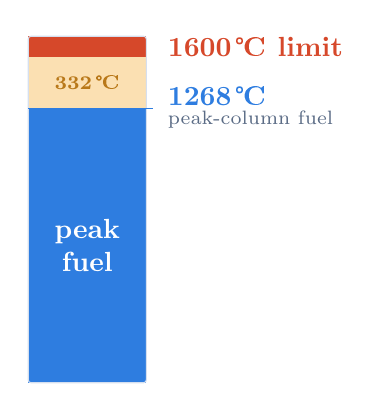
\begin{tikzpicture}[font=\scriptsize]
  \def\H{4.4}\def\W{1.5}
  \pgfmathsetmacro\pk{\H*0.7925}         % 1268 of 1600
  \pgfmathsetmacro\lim{\H-0.26}          % top of the amber, base of red band
  % peak fuel (blue) fills from the base up to 1268
  \fill[RadBlue] (0,0) rectangle (\W,\pk);
  \node[text=white, font=\bfseries, align=center] at (\W/2,\pk/2) {peak\\fuel};
  % margin (amber headroom) from 1268 up to the limit
  \fill[RadAmber!35] (0,\pk) rectangle (\W,\lim);
  \node[text=RadAmberD, font=\bfseries\scriptsize] at (\W/2,{(\pk+\lim)/2}) {332\,\textcelsius};
  % limit band (red) at the top
  \fill[RadHot] (0,\lim) rectangle (\W,\H);
  % outline
  \draw[rounded corners=1pt, draw=RadLine] (0,0) rectangle (\W,\H);
  % right-side callouts
  \node[anchor=west, text=RadHot, font=\bfseries] at (\W+0.15,{(\lim+\H)/2}) {1600\,\textcelsius\ limit};
  \draw[RadBlue, dashed] (0,\pk) -- (\W+0.1,\pk);
  \node[anchor=west, text=RadBlue, font=\bfseries] at (\W+0.15,\pk+0.15) {1268\,\textcelsius};
  \node[anchor=west, text=midGray] at (\W+0.15,\pk-0.15) {peak-column fuel};
\end{tikzpicture}\\[5pt]
{\color{midGray}\scriptsize How close the peak gets to the 1600\,\textcelsius\ limit.}
\end{column}
\end{columns}
\end{frame}

% ============================================================
% SITUATION 2
% ============================================================
\begin{frame}{Situation --- Hottest at Full Power}
\begin{columns}[T]
\begin{column}{0.55\textwidth}
\begin{itemize}\setlength\itemsep{7pt}
  \item At trip, fission power collapses to about \hot{6\%} decay heat almost instantly.
  \item The graphite block keeps shedding stored heat to the reactor-cavity cooling system.
  \item So the peak is the operating value, reached at cooldown onset. The block cools monotonically after that.
\end{itemize}
\end{column}
\begin{column}{0.45\textwidth}
\centering
\vspace{6pt}
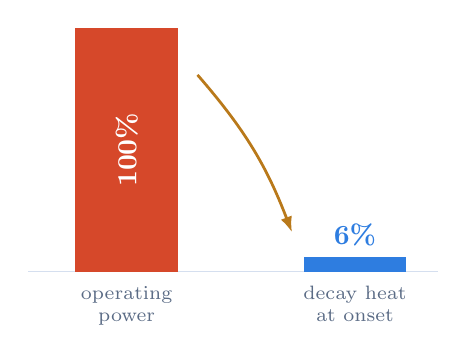
\begin{tikzpicture}[font=\scriptsize]
  \draw[RadLine] (0,0) -- (5.2,0);
  \fill[RadHot] (0.6,0) rectangle (1.9,3.1);
  \node[text=white, font=\bfseries, rotate=90] at (1.25,1.55) {100\%};
  \node[below, text=midGray, align=center] at (1.25,-0.06) {operating\\power};
  \fill[RadBlue] (3.5,0) rectangle (4.8,0.186);
  \node[above, text=RadBlue, font=\bfseries] at (4.15,0.2) {6\%};
  \node[below, text=midGray, align=center] at (4.15,-0.06) {decay heat\\at onset};
  \draw[-{Latex[length=2mm]}, RadAmberD, line width=1pt] (2.15,2.5) to[bend left=10] (3.35,0.5);
\end{tikzpicture}\\[4pt]
{\color{midGray}\scriptsize Power falls about 33-fold at trip.}
\end{column}
\end{columns}
\end{frame}

% ============================================================
% TASK
% ============================================================
\begin{frame}{Task --- Scope}
\begin{columns}[T]
\begin{column}{0.52\textwidth}
\begin{tcolorbox}[bluebox]
\small\itshape Predict peak fuel temperatures during a passive cooldown, with the context to assess accuracy.
\end{tcolorbox}
\vspace{9pt}
{\color{RadNavy}\bfseries Scoping decisions}
\begin{itemize}\setlength\itemsep{6pt}\small
  \item One fuel block and coolant-channel column, standard HTGR practice.
  \item Validate in normal operation first, then apply the same model to the cooldown.
  \item Model the depressurised cooldown. Pressurised is core-scale, out of scope.
\end{itemize}
\end{column}
\begin{column}{0.48\textwidth}
\vspace{18pt}
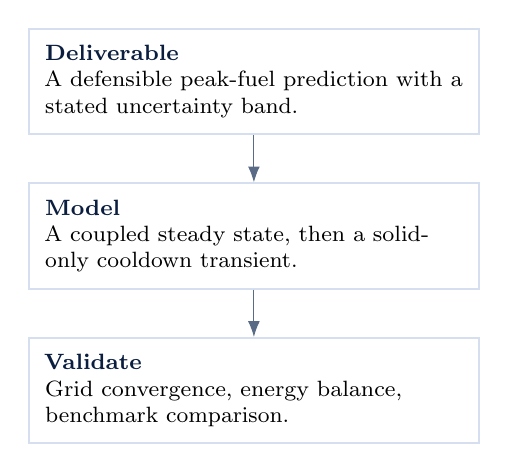
\begin{tikzpicture}[font=\footnotesize, node distance=6mm]
  \node[draw=RadLine, line width=0.7pt, fill=white, text width=5.3cm, inner sep=6pt] (g)
    {{\color{RadNavy}\bfseries Deliverable}\\ A defensible peak-fuel prediction with a stated uncertainty band.};
  \node[below=of g, draw=RadLine, line width=0.7pt, fill=white, text width=5.3cm, inner sep=6pt] (m)
    {{\color{RadNavy}\bfseries Model}\\ A coupled steady state, then a solid-only cooldown transient.};
  \node[below=of m, draw=RadLine, line width=0.7pt, fill=white, text width=5.3cm, inner sep=6pt] (v)
    {{\color{RadNavy}\bfseries Validate}\\ Grid convergence, energy balance, benchmark comparison.};
  \draw[-{Latex[length=2mm]},midGray] (g)--(m);
  \draw[-{Latex[length=2mm]},midGray] (m)--(v);
\end{tikzpicture}
\end{column}
\end{columns}
\end{frame}

% ============================================================
% ACTION 1 -- methodology
% ============================================================
\begin{frame}{Action --- Methodology}
\begin{columns}[T]
\begin{column}{0.54\textwidth}
A custom temperature-based CHT solver solves the solid directly in temperature:
\vspace{3pt}
\begin{tcolorbox}[navybox]
\centering
$\rho\,C_p(T)\,\dfrac{\partial T}{\partial t} = \nabla\!\cdot\!(\kappa\nabla T) + q'''$
\end{tcolorbox}
\vspace{4pt}
{\footnotesize The stock enthalpy formulation uses $C_p$ inconsistently: pointwise in the diffusivity $\kappa/C_p$, but interval-averaged when converting enthalpy to temperature. These cancel only for constant $C_p$, so graphite's varying $C_p$ leaves a systematic \hot{$\sim$17\,\textcelsius} error, independent of mesh.}
\end{column}
\begin{column}{0.46\textwidth}
\begin{tcolorbox}[tealbox]
{\color{RadTeal}\bfseries Steady baseline}\\[1pt]
\footnotesize Two regions, resolved helium channels coupled to the solid, marched to convergence.
\end{tcolorbox}
\vspace{5pt}
\begin{tcolorbox}[amberbox]
{\color{RadAmberD}\bfseries Passive cooldown}\\[1pt]
\footnotesize Solid only. Cooling is lost and the primary is stagnant, so helium is dropped and the channels go adiabatic. Time-accurate from the steady field.
\end{tcolorbox}
\end{column}
\end{columns}
\end{frame}

% ============================================================
% ACTION 2 -- geometry
% ============================================================
\begin{frame}{Action --- Geometry \& Mesh}
\begin{columns}[T]
\begin{column}{0.42\textwidth}
\centering
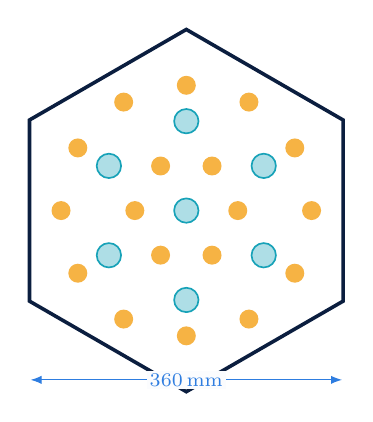
\begin{tikzpicture}[scale=0.86]
  \node[regular polygon, regular polygon sides=6, draw=RadNavy, line width=1.3pt,
        fill=white, minimum size=4.6cm, rotate=90] at (0,0){};
  \foreach \a in {30,90,...,330}{\fill[RadTeal!35, draw=RadTeal, line width=0.6pt] (\a:1.32) circle (0.18);}
  \fill[RadTeal!35, draw=RadTeal, line width=0.6pt] (0,0) circle (0.18);
  \foreach \a in {0,60,...,300}{
    \fill[RadAmber!85] (\a:0.76) circle (0.14);
    \fill[RadAmber!85] (\a:1.85) circle (0.14);
    \fill[RadAmber!85] (\a+30:1.85) circle (0.14);}
  \draw[{Latex[length=1.4mm]}-{Latex[length=1.4mm]}, RadBlue] (-2.3,-2.5) -- (2.3,-2.5)
        node[midway,fill=lightBG,inner sep=1pt,text=RadBlue,font=\scriptsize]{360\,mm};
\end{tikzpicture}\\[2pt]
{\color{midGray}\scriptsize Teal: coolant channels. Amber: fuel holes.}
\end{column}
\begin{column}{0.58\textwidth}
{\footnotesize A real MHTGR-350 cross-section extruded to a ten-block column. Fuel compacts are a heat-source zone in one graphite region, with graded near-wall refinement.}
\vspace{7pt}

{\small\renewcommand{\arraystretch}{1.25}
\begin{tabular}{@{}l r@{}}
Block across flats & 360\,mm\\
Fuel-to-coolant pitch & 18.8\,mm\\
Fuel : coolant holes & 222 : 109\\
Column height & 8.0\,m\\
Mesh & 2.64\,M cells\\
\end{tabular}}
\vspace{6pt}

{\color{midGray}\footnotesize Geometry matches the benchmark (porosity 0.186, 79.3\,cm element), cross-checked against NEA/NSC/R(2017)4\ct{1}.}
\end{column}
\end{columns}
\end{frame}

% ============================================================
% ACTION 3 -- inputs
% ============================================================
\begin{frame}{Action --- Inputs}
{\color{midGray}\footnotesize All values trace to the OECD/NEA MHTGR-350 benchmark, report NEA/NSC/R(2017)4\ct{1}.}
\vspace{8pt}

\begin{columns}[T]
\begin{column}{0.5\textwidth}
{\color{RadNavy}\bfseries Operating point}
\vspace{3pt}

{\small\renewcommand{\arraystretch}{1.25}
\begin{tabular}{@{}l r@{}}
Coolant, pressure & Helium, 6.39\,MPa\\
Inlet temperature & 259\,\textcelsius\\
Inlet velocity & 18.8\,m/s\\
Power density (fuel) & 24.8\,MW/m$^3$\\
\end{tabular}}
\vspace{7pt}

{\color{RadNavy}\bfseries Decay heat}
\vspace{2pt}

{\footnotesize ANS-5.1 curve, about 6\% at onset falling to 0.4\% at 100 hours.}
\end{column}
\begin{column}{0.5\textwidth}
{\color{RadNavy}\bfseries Materials, H-451 graphite}
\vspace{3pt}

{\small\renewcommand{\arraystretch}{1.25}
\begin{tabular}{@{}l r@{}}
Density & 1850\,kg/m$^3$\\
Emissivity & 0.85\\
Specific heat $C_p(T)$ & benchmark fit\\
Conductivity $\kappa(T)$ & un-irradiated\\
\end{tabular}}
\vspace{8pt}

\begin{tcolorbox}[hotbox]
\footnotesize Conductivity is the un-irradiated value. Irradiation lowers $\kappa$, which runs the fuel hotter, so this input under-predicts the peak. Quantified in the accuracy assessment.
\end{tcolorbox}
\end{column}
\end{columns}
\vspace{3pt}

{\color{midGray}\scriptsize Cites: spec pp.\,16--17, Tables AIV.2--AIV.3, \S\,I.7.4; full trace in \texttt{benchmark/README.md}.}
\end{frame}

% ============================================================
% ACTION 4 -- boundary conditions
% ============================================================
\begin{frame}{Action --- Boundary Conditions}
\vspace{2pt}

{\small\renewcommand{\arraystretch}{1.35}
\begin{tabular}{@{}p{3.0cm} p{4.3cm} p{4.7cm}@{}}
\toprule
\textbf{Surface} & \textbf{Steady} & \textbf{Passive cooldown}\\
\midrule
Coolant channels & coupled to solid & adiabatic\\
Outer wall & adiabatic & radiation to the RCCS sink\\
Axial ends & adiabatic & adiabatic\\
\bottomrule
\end{tabular}}
\vspace{12pt}

\begin{columns}[T]
\begin{column}{0.5\textwidth}
\begin{tcolorbox}[hotbox]
\footnotesize Placing the RCCS sink on the block itself zeroes the core radial resistance. It really belongs at the vessel boundary of a full-core model. This is the main reason the block shows no delayed peak.
\end{tcolorbox}
\end{column}
\begin{column}{0.5\textwidth}
\begin{tcolorbox}[tealbox]
\footnotesize The wall condition is effectively radiation-only ($\varepsilon = 0.85$, sink at 303\,K). Adiabatic channels trap heat, which is conservative for the peak.
\end{tcolorbox}
\end{column}
\end{columns}
\end{frame}

% ============================================================
% ACTION 5 -- assumptions
% ============================================================
\begin{frame}{Action --- Assumptions}
\begin{columns}[T]
\begin{column}{0.55\textwidth}
\begin{itemize}\setlength\itemsep{8pt}\small
  \item Single block and column, not the annular core.
  \item Un-irradiated conductivity.
  \item ANS-5.1 decay heat.
  \item Uniform power in the axial direction.
  \item Depressurised cooldown only.
\end{itemize}
\end{column}
\begin{column}{0.45\textwidth}
\vspace{6pt}
\begin{tcolorbox}[navybox]
{\color{RadNavy}\bfseries Why these hold}\\[3pt]
\footnotesize
A single symmetric block is the standard unit for prismatic-HTGR analysis: representative physics on a mesh clean enough to validate.
\vspace{4pt}\\
Un-irradiated $\kappa$ was the only value in the distributed data; its low bias is quantified in the accuracy assessment.
\vspace{4pt}\\
The depressurised case is the bounding conduction cooldown, so it needs no active-fluid model.
\end{tcolorbox}
\end{column}
\end{columns}
\end{frame}

% ============================================================
% RESULT 1 -- the prediction
% ============================================================
\begin{frame}{Result --- Prediction}
\begin{columns}[c]
\begin{column}{0.47\textwidth}
\centering
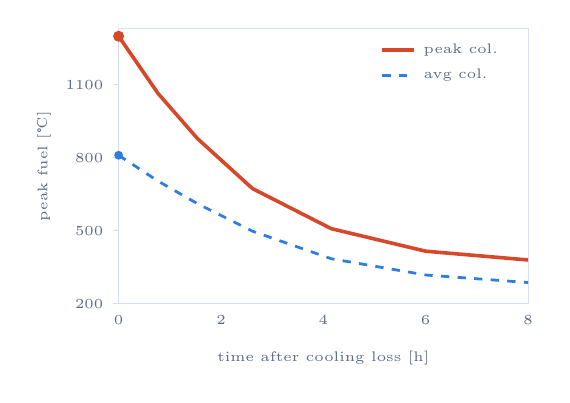
\begin{tikzpicture}[font=\scriptsize]
  \def\W{5.2}\def\H{3.5}
  \draw[RadLine] (0,0) rectangle (\W,\H);
  \foreach \y/\lab in {0/200,0.927/500,1.855/800,2.782/1100}{
     \draw[RadLine] (0,\y)--(-0.07,\y); \node[left,text=midGray,font=\tiny] at (-0.07,\y){\lab};}
  \node[rotate=90, text=midGray, font=\tiny] at (-0.95,\H/2){peak fuel [\textcelsius]};
  \foreach \x/\lab in {0/0,1.3/2,2.6/4,3.9/6,5.2/8}{
     \node[below,text=midGray,font=\tiny] at (\x,-0.02){\lab};}
  \node[below,text=midGray,font=\tiny] at (\W/2,-0.48){time after cooling loss [h]};
  % peak column 1268 -> 367
  \draw[RadHot, line width=1.3pt]
     plot coordinates {(0,{(1268-200)/1100*\H}) (0.5,{(1040-200)/1100*\H}) (1.0,{(860-200)/1100*\H})
     (1.7,{(660-200)/1100*\H}) (2.7,{(500-200)/1100*\H}) (3.9,{(410-200)/1100*\H}) (5.2,{(375-200)/1100*\H})};
  \fill[RadHot] (0,{(1268-200)/1100*\H}) circle (2pt);
  % average column 793 -> 270
  \draw[RadBlue, line width=1.0pt, dashed]
     plot coordinates {(0,{(793-200)/1100*\H}) (0.5,{(690-200)/1100*\H}) (1.0,{(600-200)/1100*\H})
     (1.7,{(490-200)/1100*\H}) (2.7,{(380-200)/1100*\H}) (3.9,{(315-200)/1100*\H}) (5.2,{(285-200)/1100*\H})};
  \fill[RadBlue] (0,{(793-200)/1100*\H}) circle (1.6pt);
  % legend
  \draw[RadHot,line width=1.3pt] (3.35,\H-0.28) -- (3.75,\H-0.28);
  \node[anchor=west,font=\tiny,text=midGray] at (3.75,\H-0.28){peak col.};
  \draw[RadBlue,line width=1.0pt,dashed] (3.35,\H-0.6) -- (3.75,\H-0.6);
  \node[anchor=west,font=\tiny,text=midGray] at (3.75,\H-0.6){avg col.};
\end{tikzpicture}\\[3pt]
{\color{midGray}\scriptsize Both columns cool monotonically from their steady peak. No delayed peak at block scale.}
\end{column}
\begin{column}{0.53\textwidth}
\begin{columns}[T]
\begin{column}{0.5\textwidth}\centering\bignum{RadHot}{1268\,\textcelsius}{peak-column fuel}\end{column}
\begin{column}{0.5\textwidth}\centering\bignum{RadNavy}{$\sim$332\,\textcelsius}{margin to the limit}\end{column}
\end{columns}
\vspace{14pt}

{\small The peak-power column (\hot{$\times$1.85}) is the bounding safety number: within 1\% of the benchmark core max (1282\,\textcelsius\ct{3}). The average column (\key{793\,\textcelsius}) validates the benchmark outlet. Both cool from their steady peak.}
\end{column}
\end{columns}
\end{frame}

% ============================================================
% RESULT 2 -- validation (steady + grid)
% ============================================================
\begin{frame}{Result --- Validation}
\begin{columns}[T]
\begin{column}{0.5\textwidth}
{\small Four meshes spanning eight-fold in cell count, average-power column.}
\vspace{5pt}

{\small\renewcommand{\arraystretch}{1.3}
\begin{tabular}{@{}l c c@{}}
\toprule
\textbf{Mesh} & \textbf{Peak fuel} & \textbf{Outlet}\\
\midrule
1.14\,M & 772.3 & 666.7\\
2.64\,M & 781.9 & 676.3\\
6.14\,M & 791.1 & 685.5\\
\textbf{9.15\,M} & \textbf{793.1} & \textbf{688.2}\\
\bottomrule
\end{tabular}}
\vspace{7pt}

{\footnotesize Converged near second order (GCI about 1\%). Coolant outlet \hot{688\,\textcelsius} against the benchmark \key{687\,\textcelsius}\ct{1}, a 0.2\% agreement.}
\end{column}
\begin{column}{0.5\textwidth}
\centering
\vspace{4pt}
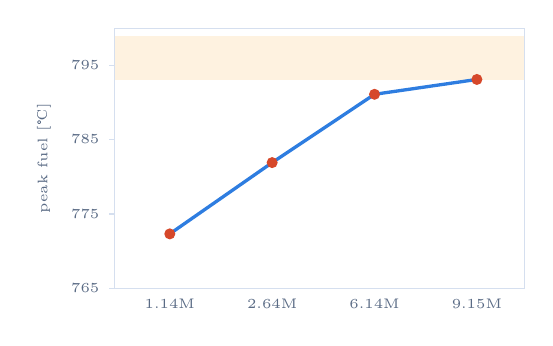
\begin{tikzpicture}[font=\scriptsize]
  \def\W{5.2}\def\H{3.3}
  \draw[RadLine] (0,0) rectangle (\W,\H);
  \foreach \y/\lab in {0/765,0.94/775,1.89/785,2.83/795}{
     \draw[RadLine] (0,\y)--(-0.07,\y); \node[left,text=midGray,font=\tiny] at (-0.07,\y){\lab};}
  \node[rotate=90, text=midGray,font=\tiny] at (-0.9,\H/2){peak fuel [\textcelsius]};
  \foreach \x/\lab in {0.7/1.14M,2.0/2.64M,3.3/6.14M,4.6/9.15M}{
     \node[below,text=midGray,font=\tiny] at (\x,-0.02){\lab};}
  \fill[RadAmber,opacity=0.14] (0,{(793-765)/35*\H}) rectangle (\W,{(799-765)/35*\H});
  \coordinate (p1) at (0.7,{(772.3-765)/35*\H});
  \coordinate (p2) at (2.0,{(781.9-765)/35*\H});
  \coordinate (p3) at (3.3,{(791.1-765)/35*\H});
  \coordinate (p4) at (4.6,{(793.1-765)/35*\H});
  \draw[RadBlue,line width=1.2pt] (p1)--(p2)--(p3)--(p4);
  \foreach \p in {p1,p2,p3,p4}{\fill[RadHot] (\p) circle (2pt);}
\end{tikzpicture}\\[3pt]
{\color{midGray}\scriptsize Peak and outlet converge together as the coolant mixing resolves.}
\end{column}
\end{columns}
\end{frame}

% ============================================================
% RESULT 3 -- verification (transient)
% ============================================================
\begin{frame}{Result --- Verification}
{\color{RadNavy}\bfseries Energy conservation over the cooldown}
\vspace{4pt}
\begin{tcolorbox}[navybox]
\centering
$\displaystyle \Delta\!\!\int_V \rho h\,dV \;=\; \int_0^t\!\!\int_V q'''\,dV\,dt \;-\; \int_0^t\!\!\oint_A \kappa\,\nabla T\!\cdot\!\hat n\,dA\,dt$
\end{tcolorbox}
\vspace{2pt}
\centerline{\footnotesize\color{midGray}stored-enthalpy change $=$ decay heat generated $-$ heat radiated to the RCCS}
\vspace{8pt}

\begin{columns}[T]
\begin{column}{0.55\textwidth}
\begin{itemize}\setlength\itemsep{6pt}\small
  \item Average column closes to \key{$<$0.25\%} ($\Delta U = -584$\,MJ), and \key{0.80\%} on the finest mesh.
  \item Peak column closes to \key{1.84\%}, a $C_p$-discretisation effect that leaves the reported peak unaffected.
  \item \key{Time-step independent}: peak fuel 778.0\,\textcelsius\ at both time steps.
\end{itemize}
\end{column}
\begin{column}{0.45\textwidth}
{\color{RadNavy}\bfseries Cooldown time constant}
\vspace{4pt}
\begin{tcolorbox}[tealbox]
\centering
$\tau = \dfrac{\rho\,c\,V}{h_\text{rad}\,A} \approx 128\ \text{min}$
\end{tcolorbox}
\vspace{4pt}
{\footnotesize CFD cooldown: \key{121\,min}, within 5\%.}
\end{column}
\end{columns}
\end{frame}

% ============================================================
% RESULT 4 -- accuracy assessment
% ============================================================
\begin{frame}{Result --- Accuracy}
{\color{midGray}\footnotesize Direction of every bias, stated for the reader.}
\vspace{7pt}

{\small\renewcommand{\arraystretch}{1.12}
\begin{tabular}{@{}p{6.2cm} p{2.8cm} p{3.4cm}@{}}
\toprule
\textbf{Source} & \textbf{Effect} & \textbf{Next step}\\
\midrule
No core radial path (block, not core) & under-predicts & effective-core model\\
Adiabatic channels & over-predicts & none needed\\
Un-irradiated conductivity & under-predicts & use irradiated $\kappa$\\
\bottomrule
\end{tabular}}
\vspace{4pt}

\begin{tcolorbox}[hotbox]
\small The average column under-predicts. Carry the peak-power column (\hot{1268\,\textcelsius}, $\approx$ benchmark core max, margin $\sim$332\,\textcelsius) as the bounding block-scale estimate. The block does not resolve the whole-core delayed peak, the next-fidelity step.
\end{tcolorbox}
\end{frame}

% ============================================================
% RESULT 5 -- limitations / next step
% ============================================================
\begin{frame}{Result --- Next Steps}
\begin{columns}[T]
\begin{column}{0.5\textwidth}
{\color{RadNavy}\bfseries What is established}
\begin{itemize}\setlength\itemsep{6pt}\small
  \item Steady baseline validated to the benchmark outlet within 0.2\%, and grid-converged.
  \item Transient integrator verified: energy-conservative and time-step independent.
  \item Every input, boundary condition, and assumption stated and traceable.
\end{itemize}
\vspace{9pt}
{\color{RadNavy}\bfseries What it is not}
\begin{itemize}\setlength\itemsep{5pt}\small
  \item It resolves one block, not the annular core, so it does not produce the whole-core delayed peak.
\end{itemize}
\end{column}
\begin{column}{0.5\textwidth}
\vspace{6pt}
\begin{tcolorbox}[bluebox]
{\color{RadBlue}\bfseries Next step}\\[2pt]
\footnotesize Restore the radial heat path with an effective-core model, moving the RCCS sink to the vessel boundary. That model can be compared directly against the benchmark full-core peak: 1391\,K\ct{2} at 50\,h, or 1237\,K at 74\,h for the ring model.
\end{tcolorbox}
\vspace{7pt}
{\color{midGray}\footnotesize This verified block model and its validated baseline are the foundation it builds on.}
\end{column}
\end{columns}
\end{frame}

% ============================================================
% SUMMARY (final content slide)
% ============================================================
\begin{frame}{Summary}
\begin{tcolorbox}[navybox]
{\color{RadNavy}\bfseries Peak fuel temperature during passive cooldown}
\vspace{3pt}

{\small\renewcommand{\arraystretch}{1.15}
\begin{tabular}{@{}l l l@{}}
& \textbf{Peak fuel} & \textbf{Margin to 1600\,\textcelsius}\\
Peak-power column ($\times$1.85, hottest) & \hot{1268\,\textcelsius} & $\sim$332\,\textcelsius\\
Average-power column & 793\,\textcelsius & $\sim$807\,\textcelsius\\
\end{tabular}}
\vspace{2pt}

{\footnotesize Steady coolant outlet 688\,\textcelsius\ (benchmark 687\,\textcelsius); peak at cooldown onset, then monotonic cooldown.}
\end{tcolorbox}
\vspace{6pt}

\begin{tcbraster}[raster columns=2, raster equal height=rows, raster column skip=6mm]
\begin{tcolorbox}[bluebox]
{\color{RadBlue}\bfseries Operating conditions}
\vspace{2pt}

{\footnotesize\renewcommand{\arraystretch}{1.2}
\begin{tabular}{@{}l r@{}}
Coolant, pressure & Helium, 6.39\,MPa\\
Core inlet & 259\,\textcelsius, 18.8\,m/s\\
Power density (avg) & 24.8\,MW/m$^3$\\
Power density (peak) & 46.0\,MW/m$^3$\\
Decay heat & ANS-5.1, $\sim$6\%\\
\end{tabular}}
\end{tcolorbox}
\begin{tcolorbox}[tealbox]
{\color{RadTeal}\bfseries Geometry}
\vspace{2pt}

{\footnotesize\renewcommand{\arraystretch}{1.2}
\begin{tabular}{@{}l r@{}}
Block & MHTGR-350 prismatic\\
Across flats & 360\,mm\\
Hole pitch & 18.8\,mm\\
Fuel : coolant holes & 222 : 109\\
Column & 8.0\,m, 10 blocks\\
\end{tabular}}
\end{tcolorbox}
\end{tcbraster}
\end{frame}

% ============================================================
% SOURCES (backup)
% ============================================================
\begin{frame}{Sources}
\vspace{10pt}
\small
{\color{RadBlue}\bfseries 1}\quad OECD/NEA MHTGR-350 benchmark, NEA/NSC/R(2017)4. Geometry, operating point, materials (Tables AIV.2--AIV.3), decay heat (\S\,I.7.4), and the steady coolant outlet (687\,\textcelsius).
\vspace{11pt}

{\color{RadBlue}\bfseries 2}\quad Strydom et al., INL. MHTGR-350 DCC/PCC transient reference results: the full-core delayed peak, 1391\,K at 50\,h (block) and 1237\,K at 74\,h (ring).
\vspace{11pt}

{\color{RadBlue}\bfseries 3}\quad MHTGR-350 steady multiphysics results: the core-maximum fuel temperature ($\approx$1282\,\textcelsius), a secondary reference band.
\vspace{16pt}

{\color{midGray}\footnotesize Benchmark values and page cites are catalogued in \texttt{benchmark/README.md}.}
\end{frame}

\end{document}
